\chapter{Analýza migrované aplikace}\label{sec:chap4}
Jako tradiční aplikace pro migraci do kontejnerové virtualizace byl zvolen OpenStack, konkrétně distribuce od firmy Mirantis, která je dodávaná jako součást produktu Mirantis Cloud Platform (MCP). Tato Aplikace by se dala označit jako tradiční aplikace, nejedná se přímo o monolitickou aplikaci, ale některými problémy je velmi tradičním aplikacím blízká. MCP distribuce byla vybrána z důvodu spolupráce s firmou Mirantis. Ta se zabývá nasazováním cloudových řešení pro enterprise zákazníky. Hlavním cílem a požadavkem ze strany Mirantisu bylo prozkoumat možnosti řešení problémů, kterými současný produkt trpí. Především otestovat principy kontejnerizace OpenStacku. V počátku této kapitoly je stručně popsán produkt MCP, poté je představena současná architektura. V závěrečné části kapitoly jsou zmíněny problémy, se kterými se platforma potýká. Součástí samotného MCP je i několik dalších podpůrných komponent Stacklight (systém pro monitoring), DriveTrain (CI/CD systém) a Ceph (storage systém). Kromě MCP existuje na trhu i řada dalších projektů a komerčních produktů postavených okolo OpenStacku, těmi nejznámějšími produkty jsou Red Hat OpenStack, SUSE OpenStack, z projektů se jedná například o TripleO, DevStack či OpenStack-Ansible. Jednotlivé produkty se pak liší v architektuře a způsobu ovládání.

\section{Mirantis Cloud Platform}
MCP je software pro tvorbu cloudových řešení. Používá se především pro privátní cloudová řešení. Celé řešení je open source, dá se tedy nainstalovat a provozovat zdarma. Hlavní byznys model je založen na podpoře a integraci platformy s okolními službami. MCP je složeno z velkého množství komponent a nabízí řešení nejen pro klasické virtuální stroje (OpenStack), ale i pro kontejnery (k8s a CaaS). V rozsahu praktické práce bude pod pojmem MCP označováno pouze OpenStack řešení bez jeho podpůrných komponent. Zbylé komponenty nejsou pro význam této diplomové práce důležité. Ovšem pro zařazení do kontextu je nutné alespoň stručně představit jednotlivé části platformy a jejich funkce.

\subsection{OpenStack}
OpenStack je software na tvorbu privátních cloudů a public cloudů, je složen z několika open source projektů, které byly postupně převedeny pod OpenStack. Projekt vznikl v roce 2010, kdy se spojila firma Rackspace Hosting s NASA a otevřely zdrojové kódy \cite{nasa_nova} ke svým projektům, ze kterých se stala nova (compute engine) a swift (object storage), a tím začal vznikat projekt OpenStack. Později začalo do projektu přispívat více kontributorů ze společností Intel, Ubuntu, Cern, IBM atd. Z OpenStacku se stal standard pro privátní cloud a předběhl i konkurenční řešení Apache Cloudstack, který je rovněž open source.

OpenStack nabízí širokou škálu projektů, které řeší mnoho problémů. Jeden z projektů, který je zaměřen na jednu speciální oblast, je projekt zvaný Sahara. Projekt řeší oblast Big Dat a lze pomocí něho instalovat a spravovat nástroje pro ně určené: Hadoop, Spark atd. Projekty typu Sahara bývají používány jen zřídka v poměru k počtu instalací do datacenter. Nejpoužívanější způsob užití pro OpenStack je virtuální infrastruktura. Pod slovy virtuální infrastruktura si lze představit několik serverů (nejčastěji Linuxových), které jsou propojeny pomocí virtuální sítě. Tato síť pak může být routovaná dál po datacentru nebo může směřovat do internetu, záleží na způsobu využití cloudu. OpenStack bývá často využíván jako náhrada za komerční cloudová řešení typu VMware. K tomuto účelu se většinou používá spojení základních sedmi komponent Nova, Keystone, Neutron, Glance, Cinder, Heat, Horizon. Nova slouží ke spuštění virtuálního workladu. Keystone je služba poskytující API pro autentifikaci, autorizaci a service discovery. Glance je služba sloužící pro ukládání image pro virtuální instance. Neutron slouží k síťování a propojení jednotlivých zdrojů. Cinder je služba, pomocí které je možno připojit do OpenStacku blokovou storage. Heat je orchestrátor, který slouží k ovládání OpenStack workloadu. Základem Heatu jsou šablony, pomocí kterých lze přistupovat k workloadu IaaC přístupem. Poslední službou je Horizon, což je webové rozhraní, pomocí kterého lze ovládat všechny výše popsané komponenty.

\subsection{DriveTrain – CI/CD}
Jak již bylo zmíněno na začátku, DriveTrain je komponenta, která se stará o instalaci MCP a následný lifecycle management. Celé řešení je spuštěno ve virtuálních strojích. Nad těmito virtuálními stroji je celý CI/CD stack spuštěn v kontejnerové virtualizaci, konkrétně v Dockeru. Pro orchestraci je využit Docker Swarm, pro ukládání perzistentních dat je pak mezi CI/CD servery nainstalován souborový systém GlusterFS. DriveTrain komponenta je složena ze čtyř hlavních komponent Jenkins, Gerrit, OpenLdap a Aptly. Jenkins je CI nástroj, který původně sloužil k sestavování softwarů a spouštění jednotlivých testů, ale díky velkému množství rozšíření je možno Jenkins využít i k dalším činnostem. Dalo by se říci, že Jenkins je CI framework, který lze pomocí rozšíření přizpůsobit pro různé úkoly. V DriveTrinu se používá na instalaci a lifecycle management cloudu. Stavebním pluginem je pipeline plugin. Pipeline si lze představit jako strom propojených úloh, které jsou spuštěny v předem daném pořadí. Pipeline jsou psané v programovacím jazyce Groovy, který je velmi podobný jazyku Java, ale díky jeho syntaxi je mnohem vhodnější na skriptování. Jednotlivé pipeline jsou složeny ze dvou základních komponent: pipeline-library \cite{github_pipelib} a mk-pipelines \cite{github_mkpipelines}. Pipeline-library je repozitář obsahující funkce, ze kterých jsou následně složeny pipeline umístěné v druhém repozitáři mk-pipelines. Tyto repozitáře jsou umístěny v Gerritu spolu s metadovým modelem. Gerrit je webová aplikace sloužící jako gitový repozitář pro ukládání zdrojových kódů. Pro regulaci přístupu do Gerritu a Jenkinse pak slouží OpenLdap. OpenLdap je implementace protokolu LDAP. Aplty slouží jako lokální obraz pro debian balíčků pro případ, že by nebyly dostupné upstream repozitáře s balíčky. Je velmi časté, že zákazníci mají cloudové prostředí bez přístupu k internetu.

Správa cloudu v praxi funguje tak, že pro každou akci prováděnou na control plane cloudu, jako jsou třeba restart služby, aktualizace balíčku či obnovení záloh databáze, je napsaná pipeline. Pipeline zapouzdřuje vždy logiku předdefinované akce. Například při obnovení databáze je třeba udělat několik kroků. Je nutno ověřit, zda existují zálohy z vybraného dne, zda není aktivní MySQL služba, poté je potřeba zálohy přesunout ze zálohovacího serveru na server s databází a až následně provést obnovení databáze. V závěrečném kroku je nutno zkontrolovat funkčnost databáze, dále zkontrolovat spojení s clusterem a dostupnost databáze pro ostatní služby. Tyto všechny akce lze spustit pomocí příkazu přes shell, pipeline tyto operace zlehčuje a šetří čas, jelikož operátor nemusí být na danou akci doménový expert. Tento koncept pipeline výrazně ulehčuje práci operátorům, kteří nemusí jednotlivé akce provádět manuálně, či si psát pro každou akci shellový skript, který může potenciálně cloud poškodit.

\subsection{Stacklight – Logování a monitoring}
Pro správný chod všech serverů a služeb je nutné celou infrastrukturu monitorovat. Za tímto účelem je v MCP naimplentován monitorovací systém. Ten stejně jako CI/CD běží v Docker Swarmu. Monitoring se dá rozdělit na dvě základní části: logování a monitoring. Logování je postavené na technologiích Fluentd a Fluent bit, které běží jako daemon na všech serverech, ze kterých sbírají logy a posílají je do časové databáze Elasticsearch, kde jsou logy po dobu 30 dnů uloženy. Pro zobrazení a lepší práci s logy je nad Elasticsearchem spuštěn nástroj Kibana. Kibana je program, který slouží k vizualizaci dat z Elasticsearch. Pomocí Kibany lze pohodlně sledovat a filtrovat pomocí různých dotazů veškeré logy v reálném čase. Druhá část monitoringu je postavená na technologii Prometheus, která sbírá jednotlivé metriky ze serverů. Tyto metriky jsou do Promethea posílány prostřednictvím programu Telegraf, který je vyčítá z jednotlivých serverů a služeb. Telegraf dokáže vyčítat velkou část metrik od vytížení CPU přes procesy až po velikost volného místa na disku. Hlavním rozdílem Promethea oproti ostatním monitorovacím nástrojům je jeho architektura, je totiž založen na principu sbírání a ukládání metrik, na rozdíl třeba od populárního Nagiosu. Díky uloženým datům v databázi lze pomocí Alertmanageru, což je část Promethea, vytvářet jednotlivá upozornění. Prometheus dále obsahuje několik rozšiřujících modulů. Například integraci s různými notifikačními systémy, což znamená, že přestane-li nějaká služba pracovat, Prometheus to pomocí metriky zjistí a zašle upozornění například do Pagerduty, Slacku či na email. Pro lepší vizualizaci si lze metriky zobrazit nejen v grafickém rozhraní Promethea, ale také v Grafaně. Grafana je nástroj, pomocí kterého, jak už název napovídá, lze jednoduše s využitím JSON jazyka vytvářet grafy.

\section{Architektura}
Hardwarovou infrastrukturu pro privátní cloud lze rozdělit na dva základní typy fyzických serverů: na KVM servery a compute. Servery, na kterých jsou spuštěny služby starající se o ovládání cloudů, se nazývají control plane. A protože v MCP jsou všechny tyto služby spuštěny na virtuálních strojích pomocí KVM virtualizace, jedná se tedy o virtuální control plane. Servery, které slouží k provozu VM vytvořených OpenStackem, se označují jako compute. Pro oba typy těchto serverů (fyzické i virtuální) je používán operační systém Linux, konkrétně distribuce Ubuntu v LTS verzi. V současné době se jedná o verzi 16.04 xenial. Celé MCP řešení je postaveno na otevřeném softwaru, většinou jsou používány upstream balíčky distribuce Ubuntu, pro služby jako OpenStack jsou použity downstream balíčky, které obsahují opravy/úpravy kódu pro jednotlivé zákazníky. Tyto změny jsou pak dostupné na Mirantis GitHubu a Gerritu.

Jak již bylo zmíněno, celý control plane OpenStacku je spuštěn ve virtuálních strojích. Pro virtuální stroje bývá jako hypervisor používán KVM. Jednotlivé virtuální stroje jsou logicky rozčleněny dle svých základních rolí. K fyzickým KVM serverům bývá připojena storage, která slouží primárně pro disky virtuálních strojů. Každá role zahrnuje logickou část OpenStacku. Schéma virtuálního control plane je na obrázku \ref{fig:mcp_arch}. K ovládání Linuxových serverů, na kterých jsou spuštěny OpenStack služby, slouží VM označené jako (cfg01), které také bývá často označováno jako salt-master. Jedná se o konfigurační server, který slouží jako hlavní ovládací konzole pro konfigurační management SaltStack, kterým je ovládáno celé řešení. Je na něm uložen metadatový model, který popisuje celou infrastrukturu. Součástí cfg nody je také aplikace MaaS (Metal as a Service), která slouží především v prvotní fázi pro instalaci fyzických serverů. MaaS dokáže na jednotlivé servery nainstalovat operační systém pomocí PXE bootu. To znamená, že pro instalaci stačí ručně nainstalovat pouze jeden operační systém, na kterém je spuštěn virtuální stroj s MaaSem a salt-masterem.

První typem nodů, které jsou spouštěny, jsou control node (ctl), které slouží pro správu a komunikaci mezi jednotlivými OpenStack službami. Na nich je nainstalovaný Keystone a serverové role některých OpenStack projektů jako například Heat, Cinder či Glance. Jednotlivé služby, jakými jsou Glance či Cinder, dokáží pracovat s různými typy backendů. V MCP se pro ukládání Glance image používají dva standardní backendy, Glusterfs nebo Ceph. Pro Cinder lze pak použít opět softwarovou storage Ceph, Lvm nebo i hardwarové řešení, pokud jimi zákazník disponuje. Další typ nodů jsou database nodes (dbs). Na těchto serverech je spuštěna databáze, která uchovává všechna data o uživatelích OpenStacku a workladu, který je v OpenStacku spuštěn. Pro tento účel se používá MySQL databáze, v MCP je použito řešení Galera Cluster od firmy Percona. Galera oproti klasickému MySQLl clusteru má lepší vlastnosti (v oblastech replikace a škálování). Dalšími typy nodů, které jsou v řešení použity, jsou message nodes (msg). Ty slouží pro software RabbitMQ, který plní funkci message brookera (fronty), a veškerá komunikace mezi OpenStack službami prochází přes tuto frontu. Pro síťování jsou použity speciální dedikované nody, ty mohou mít dva odlišné názvy (ntw nebo gtw). Záleží na tom, jaké síťovací řešení je použito. Pro OpenvSwitch, dále jako OVS, jsou použity gateway nody. Samotné OVS může být nakonfigurováno v několika různých režimech. Zde záleží na modelu routování komunikace mezi jednotlivými computy. Pro správu síťování v MCP lze také použít další SDN (Software Defined Networking) řešení implementované pomocí neutron pluginů. V současnosti hlavním SDN, které je v MCP oficiálně podporováno, je řešení původem od Juniper Network, Tungsten Fabric (dříve OpenContrail). Toto řešení implementuje dva základní typy nodů (ntw), které slouží jako controllery pro SDN. Controllery slouží ke správě virtuálních sítí. Pro ukládání informací o činnostech ve virtuálních sítích slouží analytické nody (nal). Obrovskou výhodou Tungsten Fabricu v porovnání se základním neutronem jsou vlastnosti, které Tungsten Fabric nabízí. Neutron v OVS režimu tyto vlastnosti potřebuje doinstalovat, případně dokonfigurovat prostřednictvím dalších OpenStack projektů. Jedná se o služby jako FaaS (Firewall as a Service) či LBaaS (Load balancer as a Service). Posledním typem virtuálních serverů z control planu jsou proxy nody (prx). Tyto nody slouží pro externí přístup do OpenStacku. Je na nich nainstalovaný Horizon a je zde především Nginx, který slouží jako reverse proxy pro endpointy jednotlivých OpenStack služeb a zároveň je zabezpečuje pomocí certifikátů.

Speciálním typem serveru v MCP jsou OpenStack compute (cmp). Jedná se o fyzické servery, které jsou výkonnější než KVM a je na nich spouštěn OpenStack workload – VM spravované OpenStackem. OpenStack podporuje pro compute mnoho typů hypervisorů a různé typy virtualizace, například Hyper-V, VMware vSphare či LXC. V praxi pak bývá pro virtualizaci používáno klasické QEMU/KVM. Jedná se o nejrozšířenější typ linuxové virtualizace, pro jeho používání není nutná licence pro hypervisora. Ke compute bývá často připojovaná i bloková storage, která slouží k uchování perzistentních volume pro disky instancí. Nejčastěji je pro tento typ storage v MCP využit Ceph, který dokáže poskytnout jak blokovou storage, tak i ephemeral disky. Tento typ disku je možno použít jako boot disk instance vytvořené OpenStackem.

\begin{figure}[H]
\begin{centering}
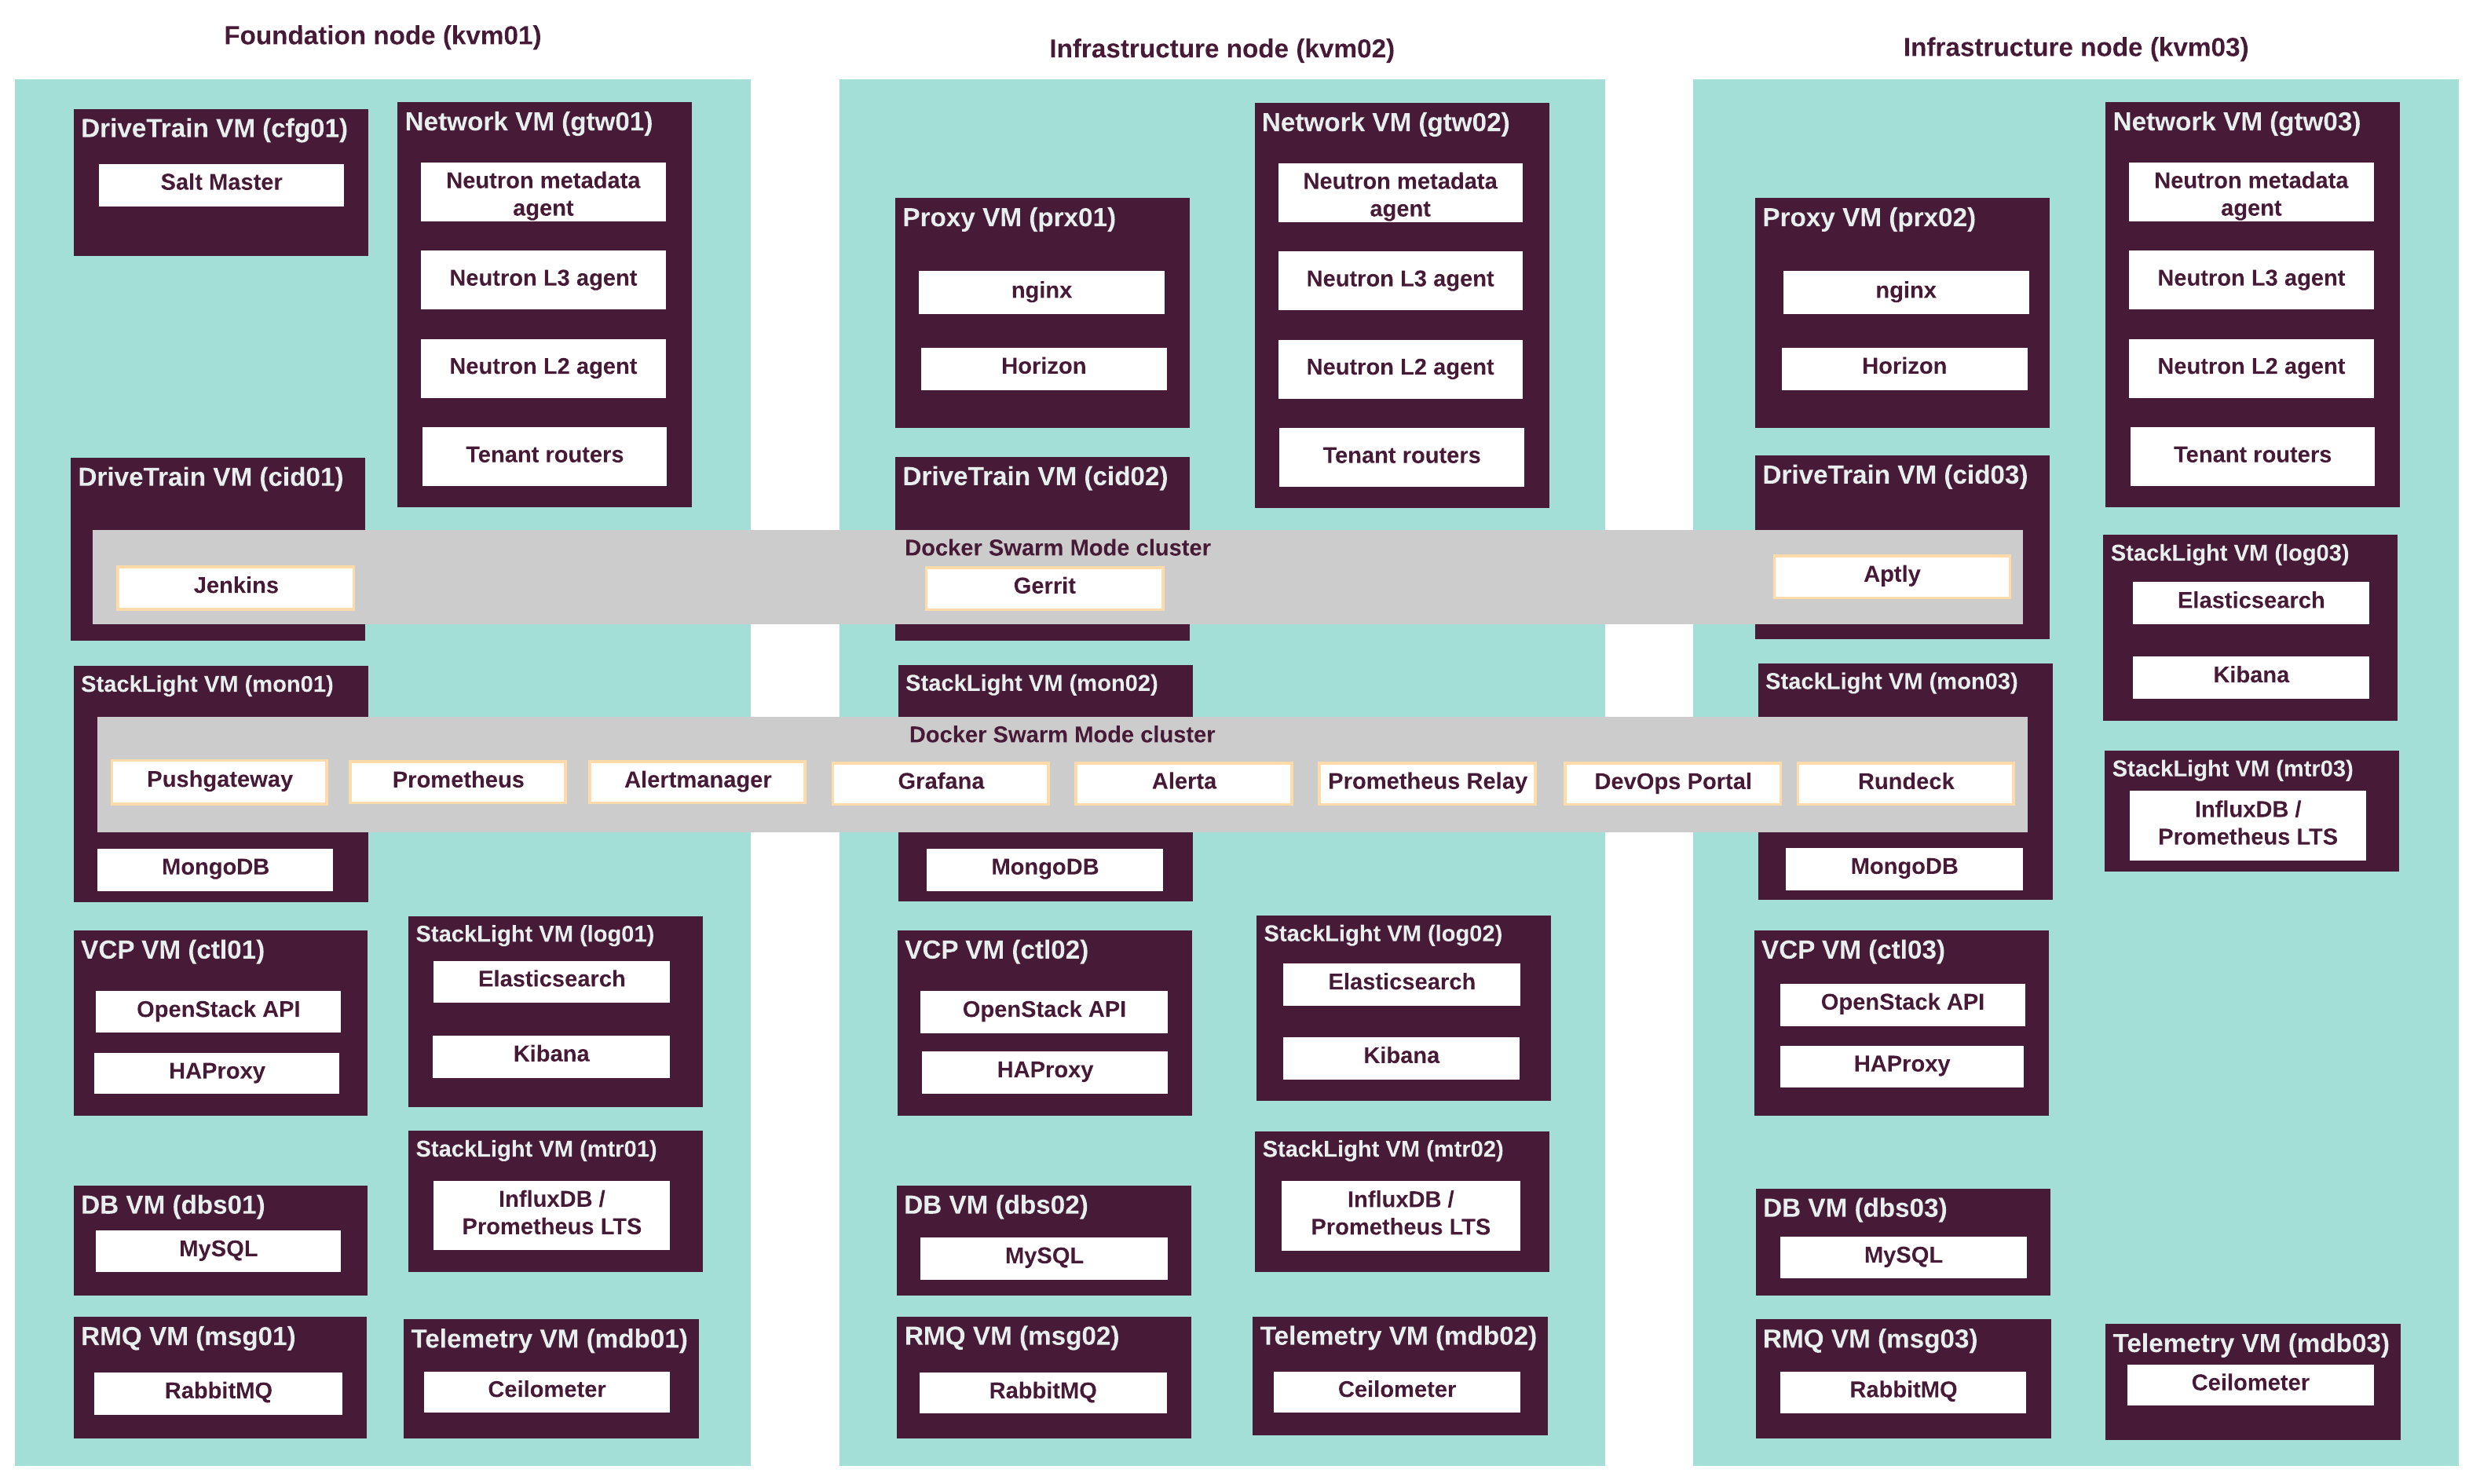
\includegraphics[width=1\textwidth]{img/mcp_ovs.png}
\par\end{centering}
\caption{MCP architektura s OVS networkingem, zdroj: \cite{mcp_arch_comp}} \label{fig:mcp_arch}
\end{figure}

Pro zajištění vysoké dostupnosti jsou všechny control plane servery spuštěny ve více replikách pro případ, že by se některá služba stala nedostupnou. Počet replik se odvíjí od počtu compute nodů v OpenStacku. Vysoká dostupnost je řešena pomocí dvou služeb, Keepalived a Haproxy. Služby jsou nakonfigurované tak, že Keepalived vytvoří virtuální ip adresu (VIP) vždy pro jeden set nodů, například control. Jednotlivé služby vždy komunikují přes VIP a daný port. Jednotlivé requesty jsou rozdělovány pomocí Haproxy mezi jednotlivé servery. Pokud jedna služba na serveru přestane fungovat, chod nebude ovlivněn, protože Haproxy bude stále rozdělovat požadavky mezi zbývající dva. Pokud je ztracen nod, který má aktivní VIP, Keepalived zjistí pomocí broadcastu, že nod nereaguje a adresa není dostupná. VIP se poté přepne na další dostupný server, záleží na prioritě, kterou má nakonfigurovanou v konfiguračním souboru.

\subsection{Orchestrace (SaltStack)}
SaltStack je software pro konfigurační management, který používá deklarativní přístup, což znamená, že vždy popisuje stav, v jakém má být prostředí či software nakonfigurován. Jednotlivé akce, které má SaltStack vykonat, jsou popsané pomocí stavů. Jednotlivé stavy jsou složeny z modulů. Tyto moduly jsou součástí SaltStacku a napsány v programovacím jazyce Python, díky tomu lze jednotlivé formule jednoduše rozšířit o další externí moduly. Veškerá instalace a konfigurace je v MCP prováděna pomocí tzv. formulí, což je sada stavů zapouzdřená do jedné logické složky. Formule pro tyto stavy může využívat různé externí moduly. Řada těchto modulů je předdefinována přímo v SaltStacku. Jedná se především o moduly pro ovládání základních služeb či moduly pro běžné akce na souborovém systému. Pro pokročilejší akce je nutné vytvářet vlastní moduly. V MCP jsou jednotlivá metadata a formule logicky rozděleny po službách či systémech. Například pro základní konfiguraci linuxových serverů lze použít salt-formula-linux, která umí nainstalovat a nakonfigurovat jednotlivé části systému, jako jsou síť nebo souborový systém. Služby typu ssh, ntp či nfs mají opět svou vlastní formuli. Toto rozdělení do logických částí poskytuje mnoho výhod. První z nich je rozdělení komplexity mezi jednotlivé formule. Každá se poté specializuje pouze na danou oblast a služba je mnohem lépe udržovatelná. Celkové řešení používá dohromady přes 100 různých formulí, které by se daly rozdělit do dalších několika kategorií.

\begin{itemize}
    \item Infrastrukturní (Linux, OpenSSH, Salt)
    \item Deployment služby (MaaS, Libvirt)
    \item Podpůrné služby (MySQL, Nginx, Apache)
    \item OpenStack služby (Keystone, Nova, Cinder)
    \item Kontejnerové služby (Docker, Kubernetes, Helm)
    \item mMonitoring (Elasticsearch, Kibana, Prometheus, Sensu)
    \item Integration (Jenkins, Aptly, Packer, Gitlab)
    \item Programovací jazyky (Java, Node, Python, Ruby)
\end{itemize}

V praxi je nutno na jednotlivých serverech, ať už virtuálních nebo fyzických, provést konfiguraci několika typů těchto služeb. Pro definici, jakou roli má mít každý server, je použit projekt Reclass (recursive external node classification), který rekurzivně spojí všechny yaml soubory naimportované na jednotlivé servery v modelu. Díky tomu může mít nadefinovaný nod víc typů různých metadat. Díky Reclassu lze též přetěžovat a přepisovat jednotlivé části modelu, což zaručuje velmi vysokou modelovací flexibilitu. S flexibilitou souvisí komplexnost a složitost modelů. Často se stane, že je daný Reclass parametr potřeba změnit. Parametry bývají častokrát v modelu přetěžovány, proto je velmi náročné najít místo, kde se nachází daný parametr, který je nutné přetížit. Parametry lze přebírat a přetěžovat napříč importy tříd modelu. Projekt Reclass je dostupný pro řadu dalších konfiguračních nástrojů, jako jsou Ansible či Puppet.

Jednotlivé salt-formule jsou vyvíjeny jako open source. Důvodem, proč byly vytvořeny nové formule a nebyly použity komunitní spravované samotným SaltStackem, jsou jednotná metadata. Formule pod hlavičkou SaltStacku (na GitHubu jako SaltStack-formulas) jsou tvořeny komunitou okolo technologie a nemají žádnou pevnou strukturu. Při nasazení většího množství formulí dohromady je nutné mít pro větší přehlednost jednotný styl metadat. V MCP je tedy využíván projekt salt-formula, který je řízen převážně Mirantisem a komunitou používající MCP. Z počátku byl projekt vyvíjen primárně na GitHubu, po čase však bylo rozhodnuto, že formule budou přesunuty a spravovány nezávisle na GitHub komunitě. Formule jsou nyní dostupné přes systém gerrit \cite{mcp_gerrit}, který poskytuje lepší možnosti spolupráce a code review než ostatní nástroje.

\subsection{Metadata model}
Současné MCP bylo od začátku navrhováno v konceptu IaaC, infrastructure-as-a-code. Znamená to, že celé cloudové řešení je postaveno nad metadatovým modelem. Model lze lehce upravovat a pomocí něho měnit prostředí. Model je složen ze tří základních typů metadat: servisních, systémových a produktových (clustrových). Tyto tři skupiny jsou od sebe izolované, a díky tomu lze jednoduše jednotlivé typy metadat kombinovat. Model je tvořen pomocí SaltStack pillaru. Těmi je popsáno, jak mají jednotlivé služby být nainstalované a nakonfigurované. Systémová a servisní část modelu je univerzální a jsou v ní předdefinovány univerzální konfigurace a parametry, tato část modelu je pro všechny instalace postavené na MCP stejná. Cluster model je hlavní část, ve které jsou nadefinovány konkrétní parametry, které jsou pro každého zákazníka či cloud unikátní. Jedná se o parametry, jako jsou hesla, jména serverů, ip adresy či dodatečná konfigurace spojená s integracemi na další systémy. Na této úrovni metadat jsou zpravidla přetěžovány parametry, které jsou definované v systémové části modelu. Všechny soubory v modelu jsou yaml soubory. Tyto soubory jsou většinou mezi sebou provázány pomocí jednotlivých importů.

\begin{lstlisting}[caption={Metadata model pro Galera databázi, zdroj: vlastní tvorba},label={lst:model_galera}]
classes:
- system.linux.system.repo.mos9
- system.linux.system.repo.saltstack
- system.galera.server.cluster
- system.galera.server.database.aodh
- system.galera.server.database.ceilometer
- system.galera.server.database.cinder
- system.galera.server.database.glance
- system.galera.server.database.grafana
- system.galera.server.database.heat
- system.galera.server.database.keystone
- system.galera.server.database.nova
- system.galera.server.database.neutron
- cluster.cloudlab_cluster
parameters:
  _param:
    keepalived_vip_interface: eth1
    keepalived_vip_virtual_router_id: 80
    galera_server_cluster_name: cloudlab_cluster
    cluster_vip_address: ${_param:openstack_database_address}
    cluster_local_address: ${_param:single_address}
    cluster_node01_hostname: dbs01
    cluster_node01_address: ${_param:openstack_database_node01_address}
    cluster_node02_hostname: dbs02
    cluster_node02_address: ${_param:openstack_database_node02_address}
    cluster_node03_hostname: dbs03
    cluster_node03_address: ${_param:openstack_database_node03_address}
  linux:
    network:
      interface:
        eth2:
          enabled: true
          type: eth
          proto: staitc        
          address: ${_param:single_address}
          netmask: ${_param:control_network_netmask}
\end{lstlisting}

Na ukázce kódu číslo \ref{lst:model_galera} je znázorněn metadatový model pro Galera databázi. Tento soubor ve formátu yaml je složen ze tří základních stavebních bloků. Prvním je blok classes, který určuje yaml soubory s třídami, které budou na nodu aplikovány. Třídy by se daly přirovnat k importům klasických tříd z objektově orientovaných jazyků. Tyto třídy udávají cestu na další yaml soubory, které jsou pomocí Reclassu vyrendrovány a spojeny v jeden velký saltstack pillar. Všechny yaml soubory začínající slovem systém pak odkazují na systémový model \cite{github_model}, na část, která je stejná pro všechny cloudy. Pillary je možné následně jednotlivými formulemi aplikovat. Jednotlivé soubory tříd se mohou navzájem přetěžovat, přetěžování funguje směrem od shora dolů. Druhou složkou jsou parametry, jejichž definice začíná na řádku 16. Tyto parametry slouží převážně k přepisování parametrů z nadefinovaných tříd, v tomto případě se jedná například o konfiguraci služby Keepalived, která slouží k zajištění vysoké dostupnosti. Poslední částí je pillar, který je unikátní pro danou službu. V ukázce se jedná o konfiguraci pro linuxový interface, řádek 28. Zde je definice pro interface eth2. Tato definice pillaru pak přetěžuje, veškeré definice přicházející ze tříd uvedených v bloku classes. Na cluster modelu se takto specifikují pouze pillary, které jsou unikátní pro jednotlivá prostředí.

\subsection{Instalace}\label{sec:chap4instal}
V předchozích částech kapitoly byl představen produkt MCP a jeho komponenty. Nyní bude popsáno, jak se tento produkt nasazuje k zákazníkům. Pro instalaci projektu je nutné mít připraveny fyzické servery, které jsou navzájem propojeny třemi odlišnými sítěmi. Jednotlivé sítě mají vždy svou úlohu. První je managment, který slouží pro řízení serverů, druhý je control plane, který slouží pro komunikaci OpenStack služeb, a poslední je dataplane, což je síť, po které komunikují instance vytvořené OpenStackem. Základem každé instalace je metadatový model, který je popsán v předchozí kapitole. Ten je vygenerován interním nástrojem postaveným nad projektem Cookiecutter \cite{cookiecutter}. Cookiecutter je šablonovací systém, který umožňuje v yaml souborech používat logiku jazyku Jinja2. To umožňuje vytvářet podmínky, proměnné, parametry či cykly. Tyto parametry jsou plněny ze souboru, který je nazýván context, jenž je ve formátu JSON. Pomocí Cookiecutteru contextu je určeno, jaké budou parametry daného cloudu a jak bude cloud nakonfigurován. U parametrů jde především o ip adresy, hesla, hostname či základní konfigurace služeb. Vygenerovaný model je nutné ještě ručně upravit pro každé prostředí, protože ne všichni zákazníci mají stejnou síťovou konfiguraci serverů nebo používají jiné storage systémy pro KVM nody. Po vygenerování modelu lze přistoupit k samotné instalaci cloudu. Instalaci operačního systému Ubuntu je nutno provést manuálně, protože operační systém pro první KVM server nelze automatizovat. Manuální část se týká také síťové konfigurace, je nutné nakonfigurovat linuxové bridge, pomocí kterých je připojena síť do konfiguračního serveru. Jakmile jsou linuxové bridge připravené, lze spustit cfg server. Disk tohoto serveru je totiž vždy stejný, a proto je pro cfg01 předpřipravená image \cite{day01_image}. Této image je při spuštění předána též config.iso, která obsahuje vygenerovaný model. Libvirt si při spuštění image přečte data ze souboru config.iso a pomocí cloud-initu spustí a nakonfiguruje cfg server již podle modelu. Po spuštění cfg serveru již lze veškerou konfiguraci provádět pomocí SaltStacku. Po spuštění konfiguračního serveru je nutné nainstalovat operační systém na zbylé servery pomocí MaaSu. Ten přes síť, která je určena pro management, začne poskytovat DHCP z předem nadefinovaného rozsahu. Hardwarové servery jsou nakofigurovány tak, že se v nekonečné smyčce pokouší o PXE boot. Jakmile obdrží ip adresu, tak se zaregistrují do MaaSu. Ten dokáže pomocí PXE na operačním systém nainstalovat operační systém Ubuntu a spustit na něm cloud-init. V rámci cloud-initu se dají provádět další poinstalační úlohy. V rámci MCP to je instalace a konfigurace salt-minionu, ten spouští stavy z salt-mastera. Jakmile jsou servery zaregistrovány pod salt-masterem, může začít instalační proces, který probíhá pomocí Jenkins pipeline. Tato pipeline je spouštěna z jenkinsu, který je předinstalován na konfiguračním serveru. Na rozdíl od DriveTrain Jenkinse tento Jenkins obsahuje pouze jednu pipeline a ta slouží pouze k instalaci cloudového prostředí. Jenkins je po úspěšném dokončení pipeline zastaven a smazán. Pro kontrolu, zda je prostředí správně nainstalováno a zda jsou všechny služby dostupné, slouží projekt Rally a Tempest. Tyto projekty však bývají spouštěny prostřednictví CVP pipeline, která se nachází v již zmiňovaném DriveTrain Jenkinsovi. Tato pipeline dokáže vygenerovat HTML reporty o tom, jak jsou služby dostupné a jakou mají odezvu.

\subsection{Správa}
Udržování cloudu a lifecycle management okolo něj jsou velmi důležité. Po instalaci, pokud nejsou vyžadovány nějaké změny, je cloud pozorován skrze monitorovací systém Stacklight, který je sám schopen na základě svých upozornění ukazovat aktuální stav. Tato upozornění bývají přeposílána do zvoleného CRM systému nebo do e-mailu. Stacklight nemonitoruje pouze stavy jednotlivých služeb, ale také metriky a logy, které jsou produkovány ostatními službami. Pokud je vyžadována nějaké změna v konfiguraci cloudu, je nutné použít následující postup. Nejprve je třeba provést změnu v metadatovém modelu a vytvořit commit se změnou a nahrát změnu do gitového repozitáře s modelem. Změnu je poté nutné na straně cloudu stáhnout a aplikovat. Lze ji aplikovat pomocí Jenkins pipeline nebo manuálně ručním voláním SaltStacku. Tento postup je doporučený především kvůli přehledu, ze kterého je patrné, co se v infrastruktuře stalo a kdo změnu provedl. Z důvodu úplnosti a správnosti změn není vhodné změny dělat na konfiguračním serveru. Zejména u větších operations týmů není přehled, kdo změny vykonal a jaké změny byly na serverech aplikovány.

\section{Problémy}
I když MCP je oproti jiným cloudovým řešením od ostatních vendorů velmi flexibilní a nabízí řadu možností, které se týkají integrace a jednotlivých konfigurací, přesto se jak pracovníci Mirantisu, tak jejich zákazníci setkávají s problémy, které je nutné každodenně řešit. V počátcích OpenStacku neumělo mnoho firem OpenStack správně nainstalovat a nakonfigurovat. V současnosti se řeší spíše problémy spojené s úlohami, které se objeví až po instalaci cloudů, jako jsou bezpečností aktualizace a upgrady. Následující část bude věnována nejproblematičtějším částem MCP z pohledu vývojáře a správce.

\subsection{Složitost}
Prvním z problémů je správa cloudového řešení. Nejedná se jenom o správu workloadu, který je spravován OpenStackem, ale o samotné cloudové řešení. Problémem je jeho složitost a množství komponent, které je potřeba znát a ovládat. Open source cloudové řešení pro svou správu vyžaduje širokou znalost technologií, od databází přes operační systém Linux až po síťování. Pro takovýto technologický stack je velmi obtížné zajistit zaměstnance nebo partnery, kteří by chtěli do MCP integrovat svůj produkt. Díky vysoké učební křivce může seznámení s řešením trvat i v řádu měsíců. Každý OpenStack vendor má své řešení postaveno trošku jinak a používá k jeho orchestování odlišné nástroje. Pro koncového zákazníka je téměř nemožné tak složité prostředí udržovat a spravovat pouze vlastními pracovníky. Většina vendorů nabízí možnost placené podpory, která pomůže zákazníkům operovat služby, nad kterými je OpenStack spuštěn. Zákazník se poté stará pouze o workload a konfigurace OpenStacku samotného.

Složitost modelu se odvíjí dle požadavků jednotlivých zákazníků. Obecně platí pravidlo: čím více komponent a integrací, tím komplikovanější model. Protože cloudy jsou živé prostředí, mohou být jednotlivé modely upravovány v čase. Pro aktualizaci cloudu je nutné projít celou metadatovou strukturu. Jelikož jsou metadata uložena na souborovém systému v jednotlivých yaml souborech, je velmi těžké zajistit jejich standardizovanou strukturu. Během aktualizací se běžně stávalo, že některé komponenty nefungovaly správně, protože inženýr, který aktualizaci prováděl, přehlédl chybu v metadatovém modelu. Dalším problémem, se kterým se inženýři u zákazníků setkali, byly ručně provedené změny v konfiguračních souborech. Celé MCP řešení je totiž navrhováno tak, aby jednotlivé služby byly konfigurovatelné metadatovým modelem z jednoho místa. Pokud je v modelu odlišná konfigurace, než je na cílovém serveru, může být tato chybná změna nechtěně aplikovaná bez jakéhokoliv vědomí.

\subsection{Life cycle management a aktualizace}
Vzhledem k velkému množství rutin a repetitivních záležitostí, které jsou na MCP cloudech, se dospělo k závěru, že je nutné tento typ akce automatizovat. Aby nebylo nutné všechny příkazy volat ručně, jsou tyto akce volány skrze Jenkins pipeline. Jedná se o úlohy, jako jsou obnovení či záloha Galera databáze, výměny Ceph osd disku či aktualizace na novější MCP verzi. Lifecycle probíhal způsobem, kdy byla provedena změna v modelu a nová verze modelu byla stažena na konfigurační server. A poté byla spuštěna pipeline z DriveTrine Jenkinse. Jednotlivé pipeline volaly jednotlivé stavy z salt-formuli nebo shell příkazy, například ověření výstupu. Bohužel ne všechny úlohy jsou takto automatizované, například různé konfigurace služeb jako IDM nikdy nebyly zařazeny do pipeline a je stále potřeba provádět je přes SaltStack manuálně. Neautomatizované služby jsou především služby, které nebyly zákazníky často vyžadovány. Používáním se osvědčilo, že tato abstrakce logiky do Jenkins pipeline je vhodná pouze na jednoduché repetitivní úlohy (výše zmiňovaná výměna osd disku pro Ceph). Pro pokročilejší akce, jako jsou především aktualizace na nové verze, slouží například komponent OpenStack, Ceph či OpenContrail.

Pro tyto komponenty byla napsána univerzální pipeline. Jedním z problémů univerzální pipeline bylo přidávání možnosti aktualizovat na novější verzi. Nové verze OpenStacku přicházely se změnami, které byly těžko automaticky implementovatelné, jednalo se například o změny databázových schémat pro nové služby. Dalším problémem těchto univerzálních postupů je fakt, že zpočátku nepočítaly se zákaznickými integracemi. Ve většině případů pipeline na aktualizaci cloudu skončily neúspěšně, protože pipeline narazila na nějaký nepředvídatelný problém. Zprvu byla iniciativa upravovat aktualizační pipeline vždy pro každého zákazníka a vývojový tým musel pokaždé vytvořit totožné vývojové prostředí jako zákaznický cloud, a to včetně rozšiřujících integrací. Bohužel průběh replikace prostředí byl velmi těžkopádný a pomalý. Proto přišel nový požadavek, který měl zkusit rozumně tyto integrace v pipeline zohlednit. V praxi se ovšem jednalo o ještě složitější proces, od kterého nakonec bylo ustoupeno. Nakonec bylo rozhodnuto, že se aktualizace budou provádět pouze ručně servisní inženýrem, který má aktualizační manuál. Ten se skládá z univerzálních kroků, ze kterých pipeline vycházela. Aktualizační manuál byl složen z jednotlivých kroků, které se měly během aktualizace cloudového prostředí provádět. Tento list kroků byl následně inženýrem doplněn o další manuální kroky, které bylo nutno při aktualizaci vykonat. Nevýhodou je, že tvorba takového plně funkčního aktualizačního manuálu je časově náročná a komplikovaně škálovatelná.

\subsection{Vývoj a testování}
Problémem, který v důsledku současné složité architektury vznikl, je pomalé vydávání nových verzí platformy a doručovaní těchto verzí zákazníkům. Vývoj je prováděn pomocí malých virtuálních prostředí, vytvořených ve vývojovém cloudu postaveném také na OpenStacku. Aby vývojářům bylo umožněno co největší pohodlí, tak je vytváření labů implementováno pomocí Jenkins pipeline. Tato pipeline je tvořena ze tří hlavních částí. První je generování modelu, poté jsou vytvořeny virtuální zdroje pomocí heat šablony a závěrečný krok je spuštění instalace prostředí. Instalace probíhá pomocí další pipeline, která spouští jednotlivé salt stavy pomocí salt API. Salt API je součástí konfiguračního serveru. Tento způsob automatizace je velmi vhodný, jelikož pomocí něj lze spustit prostředí, které je v mnohých parametrech velmi identické s reálnými produkčními clustery. Navíc laby samy k instalaci používají stejnou instalační proceduru, která je používána u zákazníků. Nevýhodou těchto virtuálních labů pro vývoj je především jejich velikost. I přestože jsou laby zmenšené, zabírají velké množství zdrojů. Například i pro vývoj drobné funkcionality do linux formule je nutno spustit lab, ve kterém nebudou využity všechny komponenty.

Samotné testování je tvořeno dvěma základními druhy. Prvními testy, kterým změny či opravy procházejí, jsou zabudované CI testy. Testují především syntaxi a možnost sestavení instalačního balíčku, tato část testování je prováděna automaticky Jenkinsem po commitu. Hlavní testování přichází při testování komponenty. To bývá prováděno na úrovni vývojového týmu, kdy je testována funkčnost požadovaných změn či vlastností komponenty. Druhý druh testování je nazýván integrační a slouží k testování jednotlivých komponent a změn najednou. Tyto integrační testy jsou dále rozděleny do tří skupin: testování na virtuálních labech, fyzickém hardware a tzv. scale testování. Integrační testování bývá prováděno speciálním QA týmem, který má k dispozici již hardwarové zdroje. Nevýhodou celého tohoto cyklu je doba testování chyb a nových vlastností. Každá změna musí být před svým zařazením do nové verze otestována s ostatními komponentami, většina nových vlastností vyžaduje i ruční kontrolu. Testování jedné malé změny může zabrat i několik hodin času QA inženýra.